
\documentclass{article}   
\usepackage[utf8]{inputenc}

\usepackage{color}
\usepackage{graphicx} % in the STTT example
\usepackage{amsmath}
\usepackage{amssymb}
\usepackage{mathtools}
\usepackage{algorithm}
\usepackage{multirow}
\usepackage{color}
%\usepackage{amsmath,amssymb,dsfont}
\usepackage{multirow}
\usepackage{algpseudocode}
\usepackage{algorithmicx}
\usepackage{float}
\addtolength{\topmargin}{-100pt}
\addtolength{\textheight}{160pt}

\renewcommand{\textfraction}{0.05}
\renewcommand{\floatpagefraction}{0.90}


\newcommand{\red}[1]{\textcolor{red}{#1}}
\newcommand{\blue}[1]{\textcolor{blue}{#1}}

\newcommand{\IGNORE}[1]{}

\newcommand{\ttit}[1]{{\text{\it #1}}}
\newcommand{\imgchar}[1]{{\bf\small({#1})}}
%\newcommand{\rewrite}{Rewrite}
\newcommand{\Sat}{\text{\it Sat}}
\newcommand{\SatELTL}{\text{Sat{$\exists$}LTL}}
\newcommand{\SatLTL}{\text{SatLTL}}
\newcommand{\SatCTL}{\text{SatCTL}}
\newcommand{\SatCTLstar}{\text{SatCTL*}}
\newcommand{\satCTL}{\Call{satCTL}}
\newcommand{\satLTL}{\Call{satLTL}}
\newcommand{\satELTL}{\Call{sat{$\exists$}LTL}}
\newcommand{\rewrite}{\Call{rewrite}}
\newcommand{\tuple}[1]{{\langle{#1}\rangle}}
\newcommand{\CTLstarMEDD}{{\small RGMEDD*}}
\newcommand{\RGMEDD}{{\small RGMEDD3}}
\newcommand{\ltsmin}{LTSmin}
\newcommand{\greatspn}{GreatSPN}
\newcommand{\meddly}{Meddly}
\newcommand{\spot}{Spot}
\newcommand{\Paths}{\mathbf{\cal P}}
\newcommand{\place}[1]{#1}
\newcommand{\trans}[1]{#1}
\newcommand{\Lang}{\mathcal L}
\newcommand{\AP}{AP}


\newcommand{\PsiRule}{\boldsymbol\Psi}
\newcommand{\phiRule}{\boldsymbol\phi}
\newcommand{\varphiRule}{\boldsymbol\varphi}
\newcommand{\doubleAmp}{\ensuremath{\mathop{\scalebox{0.80}{\&\!\&}}}}
\newcommand{\doublePipe}{\ensuremath{\mathop{\scalebox{0.80}{$||$}}}}

\begin{document}
\title{Esercizio Reti di Petri Produttori e Consumatori}
\author{Lorenzo Dentis}

\date{\today}

\maketitle

\section{Primo setting: 1 produttore, 1 consumatore, 1 buffer a N posizioni}\label{SEC:primo}
La Petri Net in Figura \ref{FIG:setting1} mostra una basilare rete "producer-consumer" divisibile in 3 sezioni.
\begin{itemize}
	\item Buffer: il buffer ad accesso casuale ad N posizioni è implementato tramite due posti, \emph{buffer} e \emph{buffer\_capacity}.Il primo svolge il ruolo di limite minimo, quanti prodotti sono presenti all'interno del buffer; il secondo fa da limite massimo, impedendo che il produttore inserisca più di N elementi.
	\item Producer: Il produttore genera l'elemtento e lo inserisce nel buffer tramite la transizione \emph{place}, tale transizione non è abilitata se non sono presenti token nel posto \emph{buffer\_capacity}, cioè il buffer è pieno
	\item Consumer: Il consumatore preleva un elemento dal buffer (solo se è presente un token nel posto \emph{buffer}) e lo "consuma".
\end{itemize}
Il reachability graph mostra un totale di 8 markings quando $N =1$, il numero di markings aumenta linearmente rispetto al valore $N$.\begin{center}$markings = 4*N + 8$\end{center}
\begin{figure*}[!h]
\centering
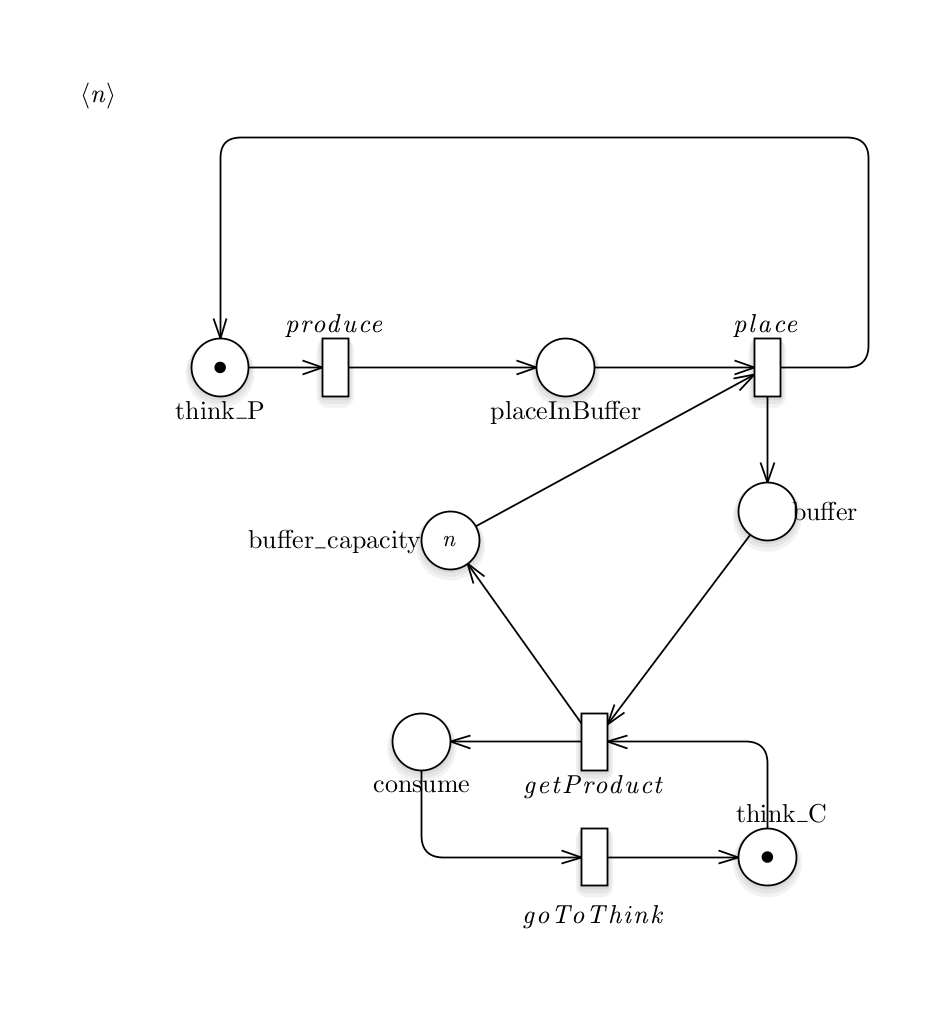
\includegraphics[width=0.75\textwidth]{./Esercizio2_img/setting1.png}
\caption{Setting 1} \label{FIG:setting1}
\end{figure*}


\section{Secondo  setting: 1 produttore, 2 consumatori,  1 buffer a N posizioni}\label{SEC:secondo}
\subsection{Secondo  setting: scalatura di marcatura}\label{SEC:secondo-marking}
La soluzione con la scalatura di marcatura richiede di modificare la marcatura del posto \emph{Think\_C}, portando il numero di token a due.\\
L'implementazione è triviale ed il numero di markings mantiene una relazione di linearità rispetto ad $N$. per quanto la costante di proporzionalità sia superiore rispetto al caso precedente non vi è un eccessivo incremento di markings anche con valori di $N$ alti. Ad esempio con $N = 1$ il reachability graph presenta 12 markings mentre con $N = 30$ ne sono presenti 182.\\
La figura \ref{FIG:setting2_markdown} mostra la rete di Petri risultante, praticametente identica alla rete tratta nella sezione precendente \ref{FIG:setting1}\\\begin{center}$markings = 6*N + 12$\end{center}
\begin{figure*}[!h]
\centering
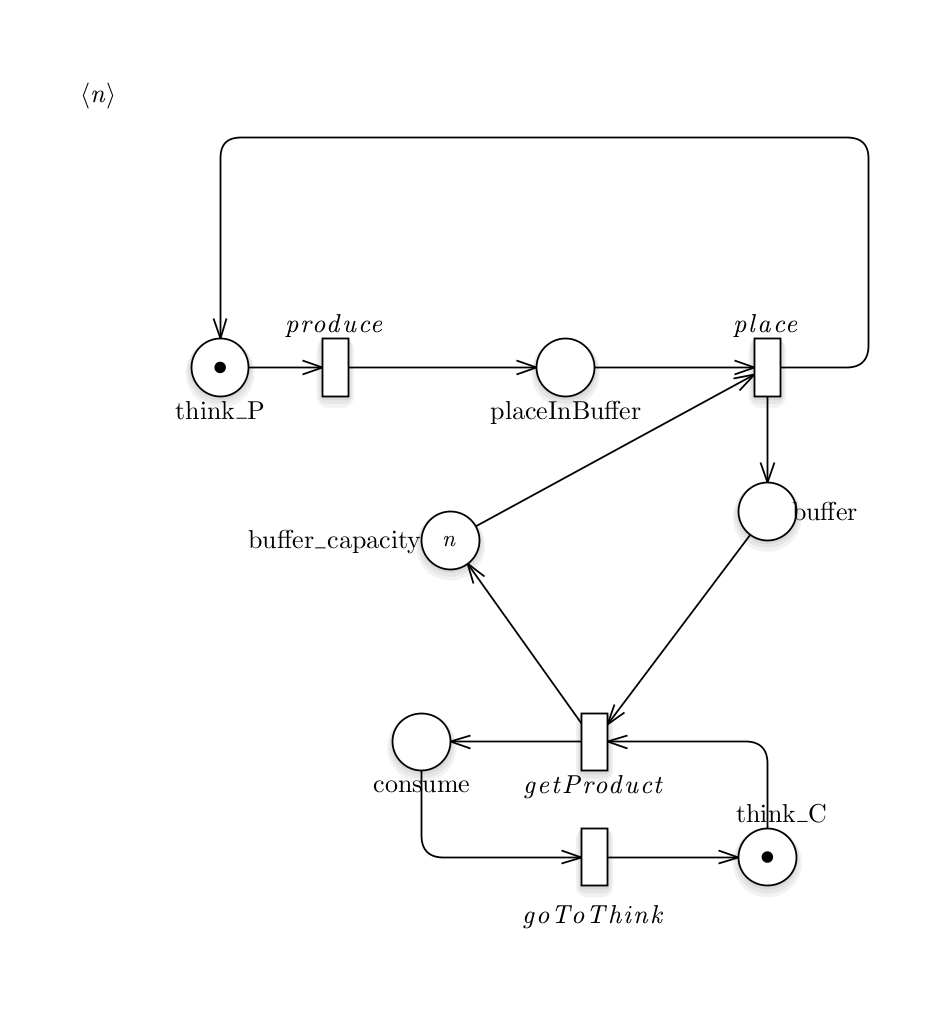
\includegraphics[width=0.75\textwidth]{./Esercizio2_img/setting1.png}
\caption{Setting 2 con scalatura di marking} \label{FIG:setting2_markdown}
\end{figure*}

\subsection{Secondo  setting: replicazione di sottoreti}\label{SEC:secondo-replica}
La soluzione tramite la replicazione della sottorete consumatore 


\section{Terzo  setting: $P$ produttori, $C$ consumatori,   1 buffer a N posizioni}\label{SEC:terzo}
\subsection{Terzo  setting: scalatura di marcatura}\label{SEC:terzo-marking}
\subsection{Terzo  setting: replicazione di sottoreti}\label{SEC:terzo-replica}


\end{document}
